\chapter{State-of-the-art overview} \label{sec:chapter_shallow}
In this chapter, we first introduce basic measures that are used for comparison of anomaly detectors. Then, we describe the current stat-of-the-art of anomaly detectors that are not based on generative models, since those are described in Chapter~\ref{sec:chapter_survey}.

\section{Comparing anomaly detectors}
Comparing different models on the same set of data is a basic requirement in practical and research problems. As already mentioned at the beginning of the previous chapter, anomaly detection has some common ground with binary classification tasks. Therefore, we can readily apply the evaluation metrics that are used to evaluate these tasks in comparisons of anomaly detectors. However, there are specifics of anomaly detection problems, mainly the often encountered large imbalance of labeled normal and anomalous samples, that we have to keep in mind. Also, with one exception, all the metrics that will be described here require at least some labeled anomalous samples, no matter how difficult it might be to obtain them. A more complete overview with some experimental results can be found in~\cite{vskvara2023auc}.

\begin{table}
\centering
    \begin{tabular}{c | c c}
        true label/estimated label & normal & anomalous \\
        \hline
        normal & tn & fp  \\
        anomalous & fn & tp 
    \end{tabular}
    \caption{A confusion matrix of a model which captures its performance by showing the total number of correctly (tp = true positives and tn = true negative) and incorrectly (fp = false positives and fn = false negatives) identified samples.}
    \label{tab:conf_ex}
\end{table}
Table~\ref{tab:conf_ex} displays a confusion table that introduces the basic concepts and notation needed below. It summarizes the performance of an algorithm with a particular threshold. In the context of anomaly detection, positive samples are anomalies, while normal samples are considered negative.

\subsubsection{AUC}
The most widely used measure in the field of anomaly detection is the area under the ROC (receiver operating characteristic) curve. The acronym AUC will be used in this text for the sake of brevity. The ROC curve is a parametric curve describing the trade-off between \textbf{true positive rate} (sometimes also called \textbf{recall}) $\text{TPR}(\tau) = \frac{\text{tp}}{\text{tp+fn}}(\tau)$ and \textbf{false positive rate} $\text{FPR}(\tau) = \frac{\text{fp}}{\text{fp+tn}}(\tau)$ for different values of the decision threshold $\tau$. 

Then, the area under the curve is calculated as the following integral
\begin{equation} \label{eq:auc}
\text{AUC}=\int_{\mathbb{R}}\text{TPR}(\tau)d\text{FPR}^{\prime}(\tau)d\tau = \int_0^1\text{TPR}(\text{FPR})d\text{FPR}.
\end{equation}
The last integral that uses $\text{TPR}(\cdot)$ as a function of the corresponding FPR shows the simple concept behind the AUC that can be easily discerned from a ROC curve drawn in a graph, see Fig.~\ref{fig:ROC}. An AUC value of 1.0 is equal to perfect classification/ordering of the data, while a value of 0.5 is equal to classifying by random guessing. In practice, the corresponding AUC is estimated from an empirical ROC curve using some numerical integration scheme, e.g. the trapezoidal rule.

As mentioned above, the main advantage of AUC is that it does not depend on the choice of a particular decision threshold. Also, the measure has a straightforward interpretation -- it is an estimate of the probability that a randomly chosen positive sample is ranked higher than a randomly chosen negative sample \cite{hand2001simple}. However, a lot of information is lost when the whole ROC curve is summarized into a single number. This is especially concerning for some applications, where the region of low false positive rates is of the principal interest. For example, in cybersecurity applications, it is usual to draw a ROC curve in logarithmic scale on the x-axis, which accentuates the low-FPR section of the ROC curve.

\begin{figure}
\centering
\begin{subfigure}[b]{0.45\textwidth} 
    \centering
    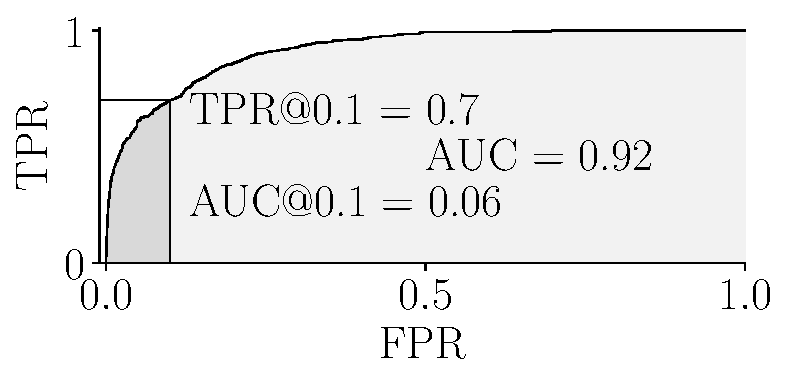
\includegraphics[width=\textwidth]{data/chapter_intro/roc_example.pdf}
    \caption{ROC curve}
    \label{fig:roc_example}
\end{subfigure}
\hfill
\begin{subfigure}[b]{0.45\textwidth}
    \centering
    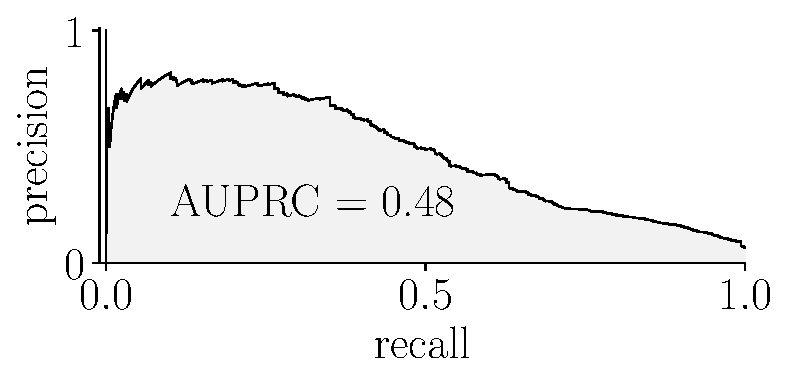
\includegraphics[width=\textwidth]{data/chapter_intro/prc_example.pdf}
    \caption{PR curve}
     \label{fig:prc_example}
\end{subfigure}
\caption{An example of a ROC curve and the derived measures captured at FPR=0.1. AUC is the whole shaded area under the ROC curve. The darker shading corresponds to AUC@0.1. On the left, the PR curve of the same detector is shown.}
\label{fig:ROC}
\end{figure}

\subsubsection{AUPRC}
The Area Under the Precision-Recall Curve is very similar to AUC, as it is given by computing the \textbf{precision} $\text{PREC}(\tau)=\frac{\text{tp}}{\text{tp + fp}}(\tau)$ and recall for different values of classification threshold $\tau$ and then integrating the area under the resulting curve. Although popular in some contexts, it has its drawbacks. A PR curve has at most as many unique recall values as positive samples in the dataset. This is problematic for anomaly detection, where the number of anomalies is low, which leads to a very sparse estimate of the true PR curve. In fact, using the same trained anomaly detector and changing the contamination rate of a testing dataset produces highly varied AUPRC results, which then makes any analysis based on AUPRC useless when the true contamination rate is unknown. Furthermore, a correct PR curve lacks a universal starting point, unlike a ROC curve, because precision is undefined for zero recall, making the computation and normalization of the area under the PR curve and the comparison between datasets even more complicated. Nevertheless, it is a metric that is reported very often besides the AUC.

\subsubsection{Areas of low TPR}
The two already mentioned metrics put the same weight on all areas on the x-axis. This might not be always ideal for the purpose of anomaly detection, as low FPR areas might be more interesting -- after all, when reporting detected anomalies for a manual check, there is always a limit on how many samples can be realistically processed. A performance measure popular among practitioners is \textbf{\tpra}, which is simply the true positive rate evaluated at a given false positive rate $\alpha \in [0,1]$. This measure can be easily read from an ROC curve. In practice, it is necessary to interpolate the ROC curve since it has discrete values, especially for datasets with a small number of samples. 

Another alternative to AUC is the partial AUC, or \textbf{\auca}, which is the area under the ROC curve calculated only up to some value of false positive rate $\alpha \in [0,1]$
\begin{equation} \label{eq:auc_alpha}
    \text{AUC@}\alpha = \int_0^{\alpha}\text{TPR}(\text{FPR})d\text{FPR}.
    \end{equation}    
Numerically, it is again important to interpolate the ROC curve for a given $\alpha$ before computing the integral. In Fig.~\ref{fig:ROC}, AUC@0.1 corresponds to the darker gray region. \auca\ can be easily normalized by dividing by the chosen $\alpha$, in which case the best detector has $\auca = 1$ similarly to AUC.

\subsubsection{Volume of decision region}
\begin{figure}
\centering
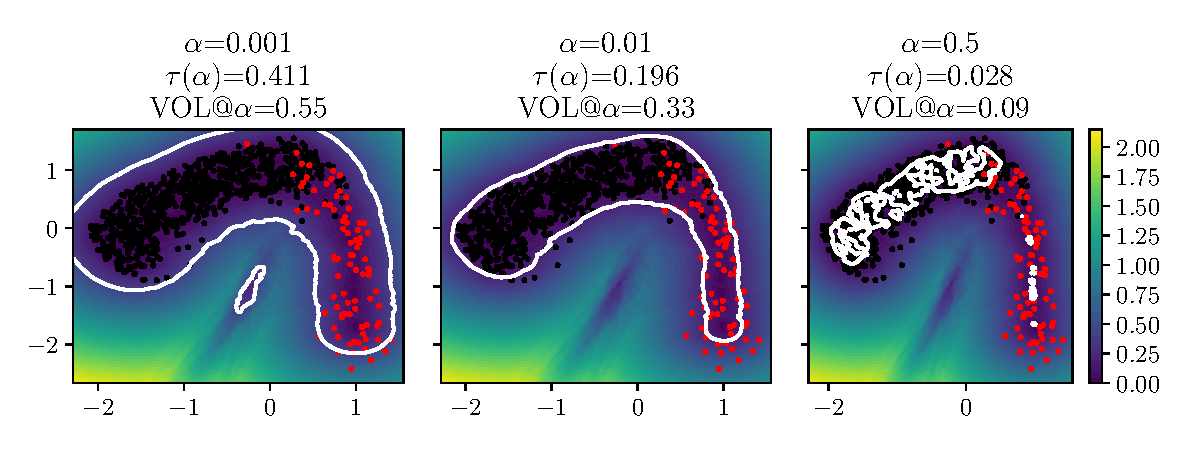
\includegraphics[scale=0.8]{data/chapter_intro/fig_vol_example.pdf}
\caption{An example of a detector and the decision region for differing values of FPR $\alpha$. The decision boundary is drawn as a white isoline at level $\tau(\alpha)$ with the estimated enclosed volume $\text{VOL@}\alpha$, black and red dots represent normal and anomalous samples in the training set. Clearly, a smaller tolerance of false positives forces us to set a higher threshold which results in higher decision region volume.}
\label{fig:vol_example}
\end{figure}
All of the previous measures originate from the evaluation of the performance of binary classifiers. Since labeled anomalies are often difficult to obtain, a measure that does not require labels for its evaluation might be more useful and better describe behaviour on unknown samples. If the goal is to compare two models supposed to characterize the normal class, and with no other assumptions about the distribution of the anomalous class, it makes sense to choose the model enclosing the training data more tightly. This corresponds to calculating the volume inside the model's decision boundary in a similar fashion to \cite{clemenccon2013scoring}, where a theoretical justification is given. This decision boundary can be chosen to correspond to a certain level of false positive rate. We define the \textbf{volume of decision region} as
\begin{equation}
  \text{VOL}(\alpha) = \int_{\mathcal{X}} \mathds{1}_{\lbrace \vc{x} \in\mathcal{X}|s(\vc{x}) <= \tau\rbrace} \left( \vc{x} \right) d\vc{x}  \text{ s.t. } \text{FPR}(\tau)=\alpha,
\end{equation}
where $\mathcal{X}$ is the input space, $s(\vc{x})$ is an anomaly score, and $\alpha \in [0,1]$ is a given false positive rate. In other words, $\text{VOL}(\alpha)$ is the volume of the subspace where the classifier returns "normal" answer with a false positive rate $\alpha$. An example of a model and its decision region for different values of $\alpha$ is shown in Fig.~\ref{fig:vol_example}. It should be noted that the idea of minimizing the enclosed volume is native to some models, e.g. the SVDD model described in Sec.~\ref{sec:domain_methods}.

Computing the empirical $\text{VOL}(\alpha)$ in data space $\mathcal{X}$ requires first finding the threshold $\tau$ corresponding to the chosen FPR $\alpha$ and then integrating the volume which corresponds to the space enclosed by the isosurface where the anomaly score is equal to $\tau$. It is numerically estimated by Monte Carlo sampling~\cite{robert1999monte}. This comes with its downsides. Mainly, the number of samples required to cover $d$--dimensional sample space grows exponentially with $d$. This issue has been addressed in \cite{goix2016evaluate}, where the volume is computed multiple times for different subsamplings of input features, however, this does not seem to be optimal as it requires training a new model for each subset of features. A comprehensive description of the practical use of this measure is presented in the original publication~\cite{vskvara2023auc}.


\section{Anomaly detectors taxonomy} \label{sec:taxonomy}
Anomaly detection methods are based on a wide range of paradigms. In this section, we will follow the taxonomy outlined in publications~\cite{pimentel2014review, ruff2020unifying}, which divide shallow (not based on neural networks) and deep (based on neural networks) detectors into groups based on their common traits. Note that this taxonomy is tentative, and some methods have traits common to multiple groups. A few examples of the most prominent methods will be given for each category, since their knowledge will be useful in the later chapters of this text, but the list is far from complete. For a complete overview of the landscape of anomaly detection methods, see the surveys~\cite{pimentel2014review, campos2016evaluation, goldstein2016comparative, moustafa2019holistic, kwon2019survey, fernandes2019comprehensive, wang2019progress, chalapathy2019deep,ruff2020unifying}.

\subsection{Probabilistic  methods} \label{sec:probabilistic_models}
Since we have defined anomaly detection as detecting samples that deviate from the normal distribution $P^+$, it is straightforward to try to model the distribution by modeling its probability distribution function (pdf). One of the simplest such methods is the Grubbs' test~\cite{grubbs1969procedures}, which assumes a Gaussian distribution of normal one-dimensional data and declares a sample to be anomalous if its distance from the mean is larger than some threshold (e.g. three standard deviations). Many such methods based on statistical tests have been proposed~\cite{barnett1994outliers}, but we will focus on advanced modeling probabilistic techniques.

\subsubsection{Shallow methods}
A \textbf{Mahalabonis distance} anomaly detector~\cite{laurikkala2000informal} is a step-up from the naive Grubbs' test as it assumes that the normal data have a multivariate Gaussian distribution. Therefore, it builds a simple parametric estimate of the normal distribution by computing the mean $\vc{\mu} \in \mathbb{R}^d$ and covariance matrix $\Sigma \in \mathbb{R}^{d \times d}$ of the training data. The anomaly score of a test point $\vc{x} \in \mathbb{R}^d$ is then
\begin{equation} \label{eq:mahalabonis_score}
    s(\vc{x}) =  (\vc{x} - \vc{\mu}) ^T \Sigma ^{-1} (\vc{x}-\vc{\mu}),
\end{equation}
which is equivalent to the evaluation of the negative log-likelihood under the Gaussian distribution. Even though this is one of the simplest and most non-robust methods, we include it here since terms similar to~\eqref{eq:mahalabonis_score} will be encountered in the remainder of this text.

\begin{figure}
	\begin{centering}
	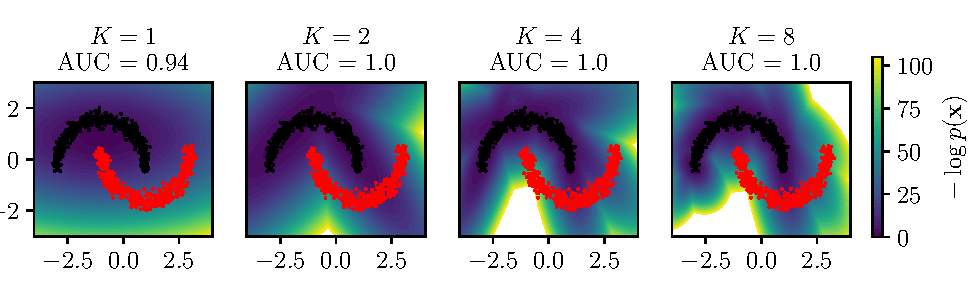
\includegraphics[scale=0.98]{data/chapter_intro/gmm_examples.pdf}
	\end{centering}
	\caption{The \textit{two bananas} dataset consists of two clusters of points. The black points are considered to be normal and the red are considered to be anomalies. The dataset is useful for introducing behaviour of anomaly detectors because as an anomaly detection problem, it cannot be solved by a linear separation of the two groups of points. Here, GMM models with a varying number of components $K$ are fitted to the normal observations. The contours of the anomaly score based on~\eqref{eq:mixture} are shown together with the AUC computed with respect to the anomalous observations.}
	\label{fig:gmm_examples}
\end{figure}
	
Instead of limiting the model to a single-mode distribution, a mixture of $K$ distributions 
\begin{equation} \label{eq:mixture}
    p(\vc{x}) = \sum_{k=1}^K p(k) p(\vc{x}|k), p(k) \in [0,1], \sum_{k=1}^K p(k) = 1,
\end{equation}
can be estimated instead, where $p(k)$ is the prior probability of the $k$-th component. \textbf{Gaussian Mixture Models} (GMMs) have been used for anomaly detection in~\cite{roberts1994probabilistic,mahadevan2010anomaly}. There, we assume that $p(\vc{x}|k)$ are Gaussian distribution densities, and their parameters are estimated using the EM algorithm~\cite{dempster1977maximum} or via Variational Bayes~\cite{bishop2006pattern}. The expression $-\log p(\vc{x})$ is usually used as the anomaly score, although sometimes the maximum of the Mahalabonis distance~\eqref{eq:mahalabonis_score} over the $K$ components is used instead. However, the viable usecases for a GMM anomaly detector are limited, mainly due to the need to compute and invert the covariance matrix, which is $O(d^3)$ in the size of the input space $d$ (when the full covariance matrix is estimated). See Fig.~\ref{fig:gmm_examples}, where the same anomaly detection problem is solved by GMMs with a different number of components. Even though the AUC score is already perfect for two components, the difficult shape of the normal data requires more components than that to be fully covered.

Time series data anomaly detection was approached with the use of \textbf{Autoregressive Integrated Moving Average} (ARIMA) models in~\cite{roberts1994probabilistic,hoare2002line}, or using a \textbf{Hidden Markov Model} (HMM) in~\cite{yeung2003host,zhang2003new}. Both approaches offer predictions for future states of an observed system, and the anomaly score is the difference between the prediction and the actual state of the system. The problems to which these methods can be applied are encountered in medicine or computer network intrusion detection.

All the previous were examples of parametric models, where a set of parameters $\vc{\theta}$ is directly estimated. Opposed to these are non-parametric models, which are less restricting  -- e.g. they do not assume any (normal, Poisson, ...) distribution -- instead, they build a parameter-free model of the normal data. \textbf{Kernel density estimation} (KDE) method~\cite{parzen1962estimation}, which estimates an unknown univariate probability density function by an empirical estimate
\begin{equation} \label{eq:kde}
    \hat{p}(x) = \frac{1}{hn} \sum_{i=1}^n k_f \left( \frac{x-x_i}{h} \right), x_i \in X
\end{equation}
where $X = \lbrace x_1, x_2, \ldots, x_n \rbrace \subset \mathbb{R}$ is the training dataset of $n$ univariate samples, $h \in \mathbb{R}^+$ is a bandwidth parameter, and $k_f:\mathbb{R} \rightarrow \mathbb{R}^+$ is a \textbf{kernel} -- uniform, triangular, normal (which is the most often used), etc., see~\cite{wand1994kernel}. Note that this is different from kernel functions used and described in Sec.~\ref{sec:domain_methods}. KDE has been used under the name Parzen window estimate e.g. in~\cite{tarassenko1995novelty,yeung2002parzen}, where $-\ln \hat{p}(x)$ is used to score anomalies. \textbf{Histogram-based Outlier Score} (HBOS) is a method~\cite{goldstein2012histogram} for anomaly detection on multivariate data $\vc{x} \in \mathbb{R}^d$. It computes normalized histograms for each feature $x_j, j \in \lbrace 1, \ldots, d \rbrace$ independently. Then the anomaly score for an unlabeled sample $\vc{x}$ is
\begin{equation} \label{eq:hbos}
    s(\vc{x}) =  -\sum_{j=1}^d \ln \tilde{p}_j(\vc{x})
\end{equation}
where $\tilde{p}_j(\vc{x})$ is the height of the bin in which $x_j$ is located. The main advantage of this method in comparison with e.g. distance-based is the relative computational simplicity. In the \textbf{Lightweight Online Detector of Anomalies} (LODA)~\cite{pevny2016loda}, an ensemble of one-dimensional histograms is used in the space of diversified projection vectors. The anomaly score is then an average of the logarithm of probabilities estimated from the histograms on individual projection vectors. Due to its simplicity and computational efficiency, it is popular in settings with high volumes of data and potentially missing input values.

\subsubsection{Deep methods}
The recent advent of neural networks has given rise to many novel methods that are more capable of handling high-dimensional datasets that would be otherwise extremely difficult to handle. A mixture model was used in the \textbf{DAGMM} method~\cite{zong2018deep}, where a neural network creates a low-dimensional latent representation $\vc{z}$ from an input $\vc{x}$. The GMM and its parameters are then estimated in the latent space, again via a neural network, which enables online learning of the whole model together.

\textbf{Energy based models} (EBMs) use the energy function $E_{\vc{\theta}}(\vc{x})$ to approximate the density as
\begin{equation} \label{eq:ebm}
    p_{\vc{\theta}}(\vc{x}) =  \frac{1}{Z(\vc{\theta})} \exp (- E_{\vc{\theta}}(\vc{x})),
\end{equation}
where $Z(\vc{\theta})$ is the partition function parametrized by $\vc{\theta}$ to ensure proper normalization of $p_{\vc{\theta}}(\vc{x})$. Although the partition function usually cannot be directly computed, an EBM can still be trained via gradient descent coupled with Markov Chain Monte Carlo estimation~\cite{hinton2002training}, which is however also the reason for its ineffectiveness relative to more novel approaches, as the MCMC is computationally costly. The anomaly score is then the energy function $E_{\vc{\theta}}(\vc{x})$. Although the direct use of the early examples of EBMs such as \textbf{Deep Belief Networks}~\cite{hinton2006fast} and \textbf{Deep Boltzmann Machines}~\cite{salakhutdinov2010efficient} was impractical for anomaly detection, they were eventually refined and successfully used on anomaly detection benchmarks in~\cite{zhai2016deep}. 

Finally, the most recent advancements in anomaly detection were achieved with the use of deep generative models that model the distribution of the data via a generative process, where it is assumed that the data is generated from a hidden latent variable. \textbf{Flow models}~\cite{dinh2014nice}, \textbf{Variational autoencoders}~\cite{kingma2013vae} and \textbf{Generative Adversarial Networks}~\cite{goodfellow2014gan}  are described in greater detail in Chapter~\ref{sec:chapter_survey}.

\subsection{Distance-based methods} \label{sec:distance_methods}
\begin{figure}
	\begin{centering}
	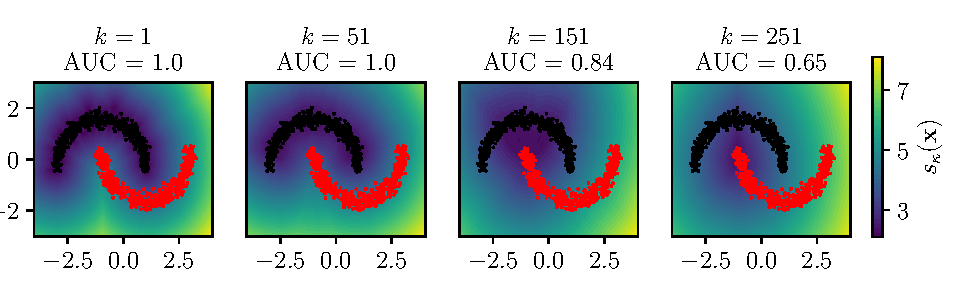
\includegraphics[scale=0.98]{data/chapter_intro/knn_examples.pdf}
	\end{centering}
	\caption{K-nearest neighbor detectors on the \textit{two bananas dataset}. The contours of the score~\eqref{eq:knn_kappa} are shown for different values of $k$ together with the resulting AUC.}
	\label{fig:knn_examples}
\end{figure}

Instead of modeling the probability distribution of the normal data, distance-based anomaly detectors use heuristics that compute a similarity measure between two data points. One of the simplest such models is the \textbf{k-Nearest Neighbor} (kNN)~\cite{ramaswamy2000efficient} model where the anomaly score of a sample is based on its proximity to its $k$-nearest neighbours from the training dataset. Consider set $X_{k}(\vc{x})$ of the $k$-nearest neighbors of $\vc{x}$ from a training dataset $X = \lbrace \vc{x}_1, \vc{x}_2, \ldots, \vc{x}_n \rbrace \subset \mathbb{R}^d$. Different anomaly scores are then described in~\cite{harmeling2006outliers}, where the Euclidean distance is used as the similarity measure:
\begin{itemize}
    \item $s_{\kappa}(\vc{x})$, where the anomaly score is the distance between $\vc{x}$ and its $k$th-nearest neighbor,
    \begin{equation} \label{eq:knn_kappa}
        s_{\kappa}(\vc{x}) =  \max_{\vc{x}_i \in X_k(\vc{x})} \vert \vert \vc{x} - \vc{x}_i \vert \vert_2,
    \end{equation}
    \item $s_{\gamma}(\vc{x})$, where the anomaly score is the average distance of $\vc{x}$ to its $k$-nearest neighbors, 
    \begin{equation} \label{eq:knn_gamma}
        s_{\gamma}(\vc{x}) =  \frac{1}{k} \sum_{\vc{x}_i \in X_k(x)} \vert \vert \vc{x} - \vc{x}_i \vert \vert_2,
    \end{equation}
    \item $s_{\delta}(\vc{x})$, where the anomaly score is the length of the mean of the vectors pointing from $\vc{x}$ to its $k$-nearest neighbours,
    \begin{equation} \label{eq:knn_delta}
        s_{\delta}(\vc{x}) =  \left| \left| \frac{1}{k} \sum_{\vc{x}_i \in X_k(x)} (\vc{x}_i - \vc{x}) \right| \right|_2.
    \end{equation}
\end{itemize}
All these definitions presume that normal data lie in concentrated regions of the data space $\mathcal{X}$, according to~\eqref{eq:normal_concentration}, while anomalies lie outside of them. The kNN anomaly detector is very popular thanks to its simplicity and good performance~\cite{campos2016evaluation}. See Fig.~\ref{fig:knn_examples}, where low values of $k$ result in a very local behaviour of the model, which is suitable for this problem. The biggest disadvantage of the model is the computational cost. Even though there is no actual training procedure, the prediction complexity is $O(ndk)$. This can be ameliorated by the construction of a $k$-d tree~\cite{bentley1975multidimensional}, which partitions the space of the training data to speed-up prediction, or using GPU-based similarity search techniques such as~\cite{johnson2019billion}. Other methods, such as \textbf{REPEN}~\cite{pangLearningRepresentationsUltrahighdimensional2018}, use the kNN detector trained on low-dimensional representations of otherwise high-dimensional data produced by a deep neural network. We will make use of this approach in models in Sec.~\ref{sec:alfven} and Chapter~\ref{sec:chapter_sgvaegan}.

The \textbf{Local Outlier Factor} (LOF) algorithm~\cite{breunig2000lof} is based on comparing the local density of a sample $\vc{x}$ with the local density of its $k$-nearest neighbours. To correctly describe the way in which the density is defined and the anomaly score is computed, we use the formula~\eqref{eq:knn_kappa}. Then we define the \textit{local reachability density} as 
\begin{equation}
  \text{LRD}_k(\vc{x})=\frac{|X_k(\vc{x})|}{\sum_{\vc{x}_i\in X_k(x)} \max \lbrace s_{\kappa}(\vc{x}), \vert \vert \vc{x} - \vc{x}_i \vert \vert_2 \rbrace }.
\end{equation}
Since this is practically the inverse of an average distance between $\vc{x}$ and its neighbours, the closer the neighbours are to $\vc{x}$, the higher this approximation of local density is. Finally, anomaly score of $\vc{x}$ is given by comparing the $\text{LRD}_k$ of $\vc{x}$ and its neighbours 
\begin{equation}
  s_{\text{LOF}}(\vc{x})=\frac{\sum_{\vc{x}_i\in X_k(\vc{x})} \text{LRD}_k(\vc{x}_i)}{\text{LRD}_k(\vc{x}) |X_k(\vc{x})|}.
\end{equation}
The rationale behind the formula is that if the local density of the neighbours is higher or the local density of $\vc{x}$ is lower then it is more likely for $\vc{x}$ to be an anomaly. This method however does not scale well in number of training samples, as its complexity is even greater than that of a simple kNN detector. Methods that are similar to LOF are the \textbf{connectivity--based outlier factor} (COF)\,\cite{tang2002enhancing} or \textbf{clustering--based local outlier factor} (CBLOF)\,\cite{he2003discovering}.


A different approach is taken by the \textbf{isolation forest }(IF) model~\cite{liu2008isolation} where an ensemble of $N_t \in \mathbb{N}$ isolation trees is constructed from the training dataset. The individual trees are constructed in such a way as to isolate each individual observation from the rest of the dataset using consecutive splits on different features. Although this procedure is stochastic  (each tree splits the data differently), it is presumed that an anomaly can be generally isolated using a smaller number of splits and therefore it usually lies on a branch closer to the root of the tree. The anomaly score is then based on the depth in which a sample is represented in the tree, averaged over all trees in the ensemble. A method similar to IF is the \textbf{Partial Identification Forest} (PIDForest)~\cite{gopalanPIDForestAnomalyDetection2019}, which uses a more informed way of choosing the data features for split, favouring more informative features.

In \textbf{Angle-Based Outlier Detection} (ABOD)~\cite{kriegel2008angle} presumes that outliers lie far from clusters of normal data, therefore the viewing angle that covers a cluster of normal observations when "looking" at it from a sample $\vc{x}$ is smaller when $\vc{x}$ is anomalous. More concretely, the method computes the angles between $\vc{x}$ and all pairs of points in the training dataset, and the anomaly score is inversely proportional to the variance of these angles -- the more varied the angles are, the more likely $\vc{x}$ is close to some cluster of normal data and the anomaly score is thus lower. In the original paper, the method is lauded for the lack of hyperparameters that need to be tuned and the ability to operate in high-dimensional data spaces. However, in the experiments in Chapter~\ref{sec:chapter_comparison}, it proves to be the method with one of the slowest prediction times.

\subsection{Domain-based  methods} \label{sec:domain_methods}
Some anomaly detectors divide the data space into a normal and anomalous subspace (domain). In~\cite{ruff2020unifying}, these are labeled as domain-based, and we will follow that distinction here.

\subsubsection{Shallow methods}
In domain-based models, the data space is partitioned into subspaces by a decision boundary. Instead of estimating the density of the whole training dataset, they only consider a few samples from it, which are called \textbf{support vectors}, and which are used to define the decision boundary. A very simple example is an anomaly detector which, for a training set $X = \lbrace \vc{x}_1, \vc{x}_2, \ldots, \vc{x}_n \rbrace \subset \mathbb{R}^d$, constructs a hypersphere with center $\vc{c} \in \mathbb{R}^d$ and radius $R>0$ that encloses the training data. It is found by solving the objective
\begin{alignat}{1}
\mathclap{
    \begin{aligned}
    \min_{R,\vc{c},\vc{\xi}} R^2 & + \frac{1}{\nu n}\sum_{i=1}^n \xi_i \\
    \text{s.t.} \vert \vert \vc{x}_i - \vc{c} \vert \vert_2^2 & \leq R^2 + \xi_i, \xi_i \geq 0, \forall i
\end{aligned}
} \label{eq:hypersphere}
\end{alignat}
where $\xi_i$ are slack variables that allow some data points to lie outside of the hypersphere. The ratio of the maximum number of outliers is controlled by the variable $\nu \in (0,1]$, which is at the same time a lower bound on the number of support vectors, which are samples $\vc{x}_i$ that lie exactly on the boundary of the hypersphere. The solution to~\eqref{eq:hypersphere} is given by solving the dual problem. Notice that a simple criterion $\vert \vert \vc{x} - \vc{c} \vert \vert_2^2  \leq R^2$ already gives a decision whether the point $\vc{x}$ is already inside the sphere. To convert this to a continuous anomaly score, we can compute the distance of $\vc{x}$ from the boundary
\begin{equation} \label{eq:hypersphere_score}
    s(\vc{x}) = \vert \vert \vc{x} - \vc{c} \vert \vert_2^2 - R^2
\end{equation}
which is negative for points inside and positive for points outside the hypersphere.

Abstracting the above, one can use \textbf{kernel functions}~\cite{shawe2004kernel} to move the problem~\eqref{eq:hypersphere} from the original input space to a transformed kernel space. The kernel is a function $k_f:\mathbb{R}^d \times \mathbb{R}^d \rightarrow \mathbb{R}$, with which we associate a \textbf{feature map} $\Phi: \mathbb{R}^d \rightarrow \mathcal{F}_k$ such that the relation defined by the inner product $k_f(\vc{x},\vc{y})=\langle \Phi(\vc{x}), \Phi(\vc{y}) \rangle$ is true for all $\vc{x},\vc{y}$. The space $\mathcal{F}_k$ is a reproducing kernel Hilbert space and we choose the kernel in such a way that its dimensionality is higher than $d$. This is the basis for the \textbf{Support Vector Data Descriptor} (SVDD) anomaly detector, where the inequality condition in~\eqref{eq:hypersphere_score} is replaced by $\vert \vert \Phi(\vc{x}_i) - \vc{c} \vert \vert_2^2 \leq R^2 + \xi_i$. By solving the problem in a space of higher dimensionality, it is possible to find a decision boundary (hypersphere) for observations that would otherwise not be separable in the original space. In comparison, the \textbf{One-Class Support Vector Machine} (OCSVM)~\cite{scholkopf2001estimating} does not construct a hypersphere, but instead aims to find a separating hyperplane in the kernel space. See Fig.~\ref{fig:ocsvm_examples} for a demonstration of the OCSVM model on our toy dataset.  Unlike in traditional SVM~\cite{cortes1995support}, which is used to separate two classes in a binary classification problem, OCSVM instead aims to find a hyperplane that maximizes the separation of the majority of the training data from the origin in the kernel space. The anomaly score of an OCSVM detector is, similarly to~\eqref{eq:hypersphere_score}, the distance from the separating hyperplane. Apart from $\nu$, a very important hyperparameter of the model is the kernel scale parameter $\gamma_{\text{OCSVM}}$. Many variants of both of the presented approaches were introduced over the years, such as \textbf{Minimum Volume Ellipsoid}~\cite{van2009minimum}, \textbf{Multi-sphere SVDD}~\cite{gornitz2017support} or \textbf{Bayesian Data Description}~\cite{ghasemi2012bayesian}.

\begin{figure}
\begin{centering}
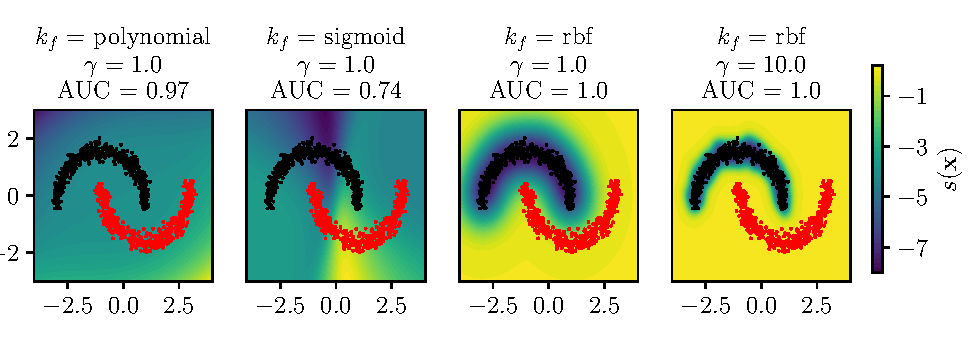
\includegraphics[scale=0.98]{data/chapter_intro/ocsvm_examples.pdf}
\end{centering}
\caption{OCSVM detectors with different kernel functions and kernel width parameter $\gamma$ values on the \textit{two bananas} dataset. The contours of the score~\eqref{eq:hypersphere_score} together with the resulting AUC are depicted. Although the use of both the polynomial and sigmoid kernels results in a relatively good AUC value, the anomaly score contours reveal that the model would fail if the anomalies were placed slightly differently. Furthermore, the tight fit of the training data with the \textit{radial basis function} (rbf) is proportional to the kernel width.}
\label{fig:ocsvm_examples}
\end{figure}

\subsubsection{Deep methods} \label{ref:sec_deep_domain}
Instead of choosing a kernel and its parameters manually, one can instead parametrize the feature maps $\Phi$ using neural networks and train them using standard gradient descent techniques, or use pre-trained networks from related tasks. This is the basis for deep OCSVM methods such as \textbf{One-class Neural Network} (OCNN)~\cite{chalapathy2018anomaly} or~\cite{erfani2016high}, or methods based on the SVDD formulation~\cite{ghafoori2020deep}. In \textbf{Deep SVDD} (DSVDD)~\cite{ruff2018deep}, the objective~\eqref{eq:hypersphere} is reformulated without the slack variables $\xi_i$, which means that the hypersphere is expected to enclose all observations in the training dataset. This simplification leads to faster convergence and yet still proves to be an effective anomaly detector. However, all the deep methods have a basic flaw. Without any further restrictions, the solution $\Phi(\vc{x}) = \vc{c}$ is valid but does not provide a useful detector. This behaviour is called the \textit{feature map collapse}. In order to prevent this, many techniques such as freezing the neural networks that provide the feature map, architectural choices or using adversarial learning are used (for an extensive list of possibilities, see~\cite{ruff2020unifying}).

\subsubsection{Training with negative examples}
Although we have stated in Sec.~\ref{sec:ad_definition} that anomaly detection methods do not usually consider the distribution of anomalies $P^-$, some approaches do. These still fall under the domain-based category of anomaly detectors, as they are mostly constructed as binary classifiers that divide the input space into subspaces where either the anomalous or normal class is expected. In the simplest case~\cite{steinwart2005classification}, $P^-$ is assumed to be uniform and a supervised classifier is trained using anomalies sampled from a hypercube centered around the normal data. This approach, however, suffers from the curse of dimensionality and saturating the hypercube in high-dimensional spaces is computationally infeasible, especially for image data. Some attempts for a more efficient sampling have been proposed, such as sampling based on local density estimation~\cite{fan2004using}. In \textbf{outlier exposure}~\cite{hendrycksDeepAnomalyDetection2019} techniques, a large auxiliary dataset, that is somehow related to normal data, is used to improve the generalization properties of a deep anomaly detector. For example, if the normal class consists of images of birds, it might be useful to train the detector to recognize normal data from images containing other animals, even though this auxiliary dataset may contain animal classes that will not be encountered as anomalies in a test/production environment. It has been shown to be an effective technique in~\cite{hendrycks2019using}.  

Outlier exposure is a form of \textbf{weak supervision}~\cite{zhou2018brief}, which is a more general term covering the approach to learning with imperfectly labeled anomaly samples. In~\cite{ruff2019deep,liznerski2020explainable} it is shown that using even a few labeled examples of anomalies can dramatically improve the detection performance. It is however important to robustify the model in order to be able to generalize to the types of anomalies not present in the labeled training dataset. These techniques can help in \textbf{active learning} in anomaly detection~\cite{abe2006outlier}, where the anomaly detector sends queries to its operator, asking for the most informative/relevant samples to be manually labeled. It is stated in~\cite{ruff2020unifying} that weak supervision is essential for potential breakthroughs in anomaly detection, which is the motivation for the method proposed in Chapter~\ref{sec:chapter_sgvaegan}.

Another paradigm where the model is trained in the presence of additional data is \textbf{self-supervision}~\cite{kolesnikov2019revisiting}, where the model solves an auxiliary task, such as prediction of transformations applied to the image~\cite{chen2020simple}. The important distinction between this approach and outlier exposure is that the transformed data is obtained from the normal training dataset by applying random translations, scalings, rotations, etc. Transforming the data in a controlled manner, the anomaly detector is then a multiclass classifier that predicts the correct transformation applied to the data. The anomaly score of such a model is then based on the softmax activations in the output layer -- if the prediction uncertainty is high, the scored sample is more likely to be an anomaly. This was very successfully used in the \textbf{Geometric Transformations} (GT)~\cite{golan2018deep} anomaly detector. Furthermore, the \textbf{GOAD} method~\cite{bergman2020classification} extends this approach to non-image data.

\subsection{Reconstruction-based methods} \label{sec:reconstruction_models}
One of the most popular approaches to anomaly detection is to build a model that learns to reconstruct input samples. When this model is trained on normal data and learns to reconstruct them well, it is expected that it will be able to identify anomalies by failing to reconstruct them properly since they have properties unseen by the model at training time. To formalize this, a reconstruction-based anomaly detector consists of an \textit{encoder}, which is a mapping $e_{\vc{\phi}}:\mathcal{X} \rightarrow \mathcal{Z}$, and a \textit{decoder} $g_{\vc{\theta}}: \mathcal{Z} \rightarrow \mathcal{X}$. Here, $\mathcal{X} \subset \mathbb{R}^d$ is the input space, $\mathcal{Z} \subset \mathbb{R}^h$ is a so called \textit{latent} space and $\vc{\phi},\vc{\theta}$ are parameters. A \textit{latent representation} or \textit{encoding} of a sample $\vc{x}$ is $z = e_{\vc{\phi}}(\vc{x})$. Reconstruction-based methods then try to match the original sample $\vc{x}$ with its reconstruction $\vc{x}' = g_{\vc{\theta}}(\vc{z})=g_{\vc{\theta}}(e_{\vc{\phi}}(\vc{x}))$. This is done by finding such parameters $\vc{\phi}, \vc{\theta}$ as to minimize the reconstruction objective
\begin{equation} \label{eq:reconstruction_objective}
    \min_{\vc{\phi}, \vc{\theta}} \vert \vert \vc{x} - g_{\vc{\theta}}(e_{\vc{\phi}}(\vc{x})) \vert \vert_2^2 + \mathcal{R},
\end{equation}
where $\mathcal{R}$ is a regularization term. Some sort of regularization is needed in order to prevent the decoding function $(g_{\vc{\theta}} \circ e_{\vc{\phi}})(\vc{x})$ to become an identity function, in which case the detector would be useless. The anomaly score of reconstruction-based methods is the \textit{reconstruction error}
\begin{equation} \label{eq:reconstruction_error}
    s(\vc{x}) = \vert \vert x - g_{\vc{\theta}}(e_{\vc{\phi}}(\vc{x})) \vert \vert_2^2.
\end{equation}


The \textbf{Principal Component Analysis} (PCA)~\cite{shyu2003novel,aggarwal2015outlier}, although not originally developed for this purpose, is an example of a reconstruction anomaly detection method. It is assumed that the normal data lie on a lower-dimensional manifold in the data space, which is an assumption also used in other methods. This means that theoretically, they can be represented by a transformation into a lower dimensional latent space, and the eventual differences between the reconstructions from the latent back to the data space and the original samples are only due to noise that is present in the data, and therefore the latent representation contains all the relevant information of a sample. PCA seeks to represent the data by finding an orthonormal basis $W \in \mathbb{R}^{h,d}$ that maximizes the empirical variance of the data $X= \lbrace \vc{x}_1, \vc{x}_2, \ldots, \vc{x}_n \rbrace \subset \mathbb{R}^d$. The original objective of PCA can be reformulated with~\eqref{eq:reconstruction_objective} in mind, which yields 
\begin{equation} \label{eq:pca}
    \max_W \sum_{i=1}^n \vert \vert \vc{x}_i -  W^TW \vc{x}_i \vert \vert_2^2, \text{s.t.} WW^T = I.
\end{equation}
Thus, this means $\vc{z} = e_{\vc{\phi}}(\vc{x}) = W \vc{x} \in \mathbb{R}^h$ is the encoding represented by the first $h$ \textit{principal components}, while the decoder is $g_{\vc{\theta}}(\vc{z}) = W^T\vc{z}$. The solution to~\eqref{eq:pca} is obtained by collecting the first $h$ eigenvectors of the covariance matrix of the training data, e.g. through its eigendecomposition, or by computing the \textit{singular value decomposition} of the data matrix. Like in the domain-based methods in Sec.~\ref{sec:domain_methods}, some of the restrictions imposed by the linear formulation of classical PCA are circumvented by using a \textbf{kernel PCA} (kPCA)~\cite{scholkopf1998nonlinear}, where $\vc{x}$ is replaced by its nonlinear transformation $\Phi(\vc{x})$. This was used for anomaly detection e.g. in~\cite{xiao2013l1}.

\begin{figure}
\begin{centering}
\begin{tikzpicture}
  \node[const]                               (x) {$\vc{x}$};
  \node[const, right = 0.5cm of x]           (xin) {};
  % encoder in
  \node[latent, right = 0.6cm of x, yshift = 0.825cm] (E11) {};
  \node[latent, right = 0.6cm of x, yshift = 0.275cm] (E12) {};
  \node[latent, right = 0.6cm of x, yshift = -0.275cm] (E13) {};
  \node[latent, right = 0.6cm of x, yshift = -0.825cm] (E14) {};
  % encoder hidden
  \node[latent, right = 1.8cm of x, yshift = 0.55cm] (E21) {};
  \node[latent, right = 1.8cm of x, yshift = 0cm] (E22) {};
  \node[latent, right = 1.8cm of x, yshift = -0.55cm] (E23) {};
  % encoder out
  \node[latent, right = 3cm of x, yshift = 0.275cm] (E31) {};
  \node[latent, right = 3cm of x, yshift = -0.275cm] (E32) {};
  % encoder tag
  \node[const, right = 2.8cm of x, yshift = 0.825cm] (E) {$e_{\vc{\phi}}(\vc{x})$};
  % code
  \node[const, right = 4.3cm of x]           (z) {$\vc{z}$};
  \node[const, right = -0.8cm of z]           (zout) {};       
  \node[const, right = 0.5cm of z]           (zin) {};
  % decoder in
  \node[latent, right = 0.6cm of z, yshift = 0.275cm] (D11) {};
  \node[latent, right = 0.6cm of z, yshift = -0.275cm] (D12) {};
  % decoder hidden
  \node[latent, right = 1.8cm of z, yshift = 0.55cm] (D21) {};
  \node[latent, right = 1.8cm of z, yshift = 0cm] (D22) {};
  \node[latent, right = 1.8cm of z, yshift = -0.55cm] (D23) {};
  % decoder out
  \node[latent, right = 3cm of z, yshift = 0.825cm] (D31) {};
  \node[latent, right = 3cm of z, yshift = 0.275cm] (D32) {};
  \node[latent, right = 3cm of z, yshift = -0.275cm] (D33) {};
  \node[latent, right = 3cm of z, yshift = -0.825cm] (D34) {};
  % xhat
  \node[const, right = 4.3cm of z]           (xhat) {$\vc{x}'$};
  \node[const, right = -0.8cm of xhat]       (xhatout) {};       
  % decoder tag
  \node[const, right = 0.6cm of z, yshift = 0.825cm] (D) {$g_{\vc{\theta}}(\vc{z})$};
  

  % edges
  \nedge {x} {xin}
  % encoder 
  \nedge {E11, E12, E13, E14} {E21, E22, E23}
  \nedge {E21, E22, E23} {E31, E32}
  % latent
  \nedge {zout} {z}
  \nedge {z} {zin}
  % decoder
  \nedge {D11, D12} {D21, D22, D23}
  \nedge {D21, D22, D23} {D31, D32, D33, D34} 
  %xhat
  \nedge {xhatout} {xhat}

  % encoder plate
%  \plate {E} {(E11)(E14)(E32)} {};
\end{tikzpicture}

\par\end{centering}
\centering{}\caption{An example of an autoencoder consisting of fully connected layers. The latent code $\vc{z}\in\mathbb{R}^{2}$ is computed by propagating the input $\vc{x} \in\mathbb{R}^{4}$ through the encoder $e_{\vc{\phi}}(\vc{x})$ and then used to produce the reconstruction $\vc{x}'\in\mathbb{R}^{4}$ via the decoder $g_{\vc{\theta}}(\vc{z})$.}
\label{fig:ae}
\end{figure}

\begin{figure}
\begin{centering}
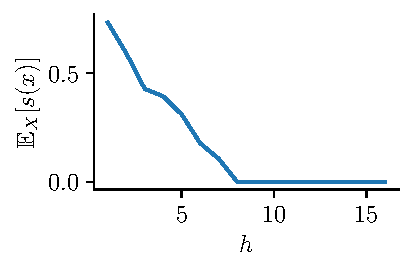
\includegraphics[scale=1.0]{data/chapter_intro/ae_reconstruction}\caption{The figure demonstrates the ability of an autoencoder to reconstruct data. The dimension $h$ of the latent space $\mathcal{Z}$ is on the x-axis, while the average reconstruction error~\eqref{eq:reconstruction_error} over the whole dataset is on the y--axis. Note that although the artificial dataset is 16--dimensional, it only contains 8 non-correlated dimensions while the remaining are a linear combination of them, which makes the data lie on an 8-dimensional manifold. This results in the error dropping to zero for $h>=8$ where the model is able to disentangle the correlations and learn the identity function.}
\label{fig:ae_reconstruction}
\par\end{centering}
\end{figure}

An \textbf{autoencoder} (AE)~\cite{kramer1991nonlinear} is in its basic principle a nonlinear PCA, where the encoder $e_{\vc{\phi}}$ and decoder $g_{\vc{\theta}}$ are neural networks and the parameters $\vc{\phi},\vc{\theta}$ are the trainable weights of these networks. The nonlinearity comes from the use of nonlinear activation functions between the individual layers of the neural networks. An example of an AE network is in Fig.~\ref{fig:ae}.  To find the weights of the neural networks, the reconstruction error ~\eqref{eq:reconstruction_error} is minimized 
\begin{equation} \label{eq:ae_objective}
\mathcal{L}_{\text{AE}}(\vc{x},\vc{\phi},\vc{\theta}) = \vert \vert \vc{x} - g_{\vc{\theta}}(e_{\vc{\phi}}(\vc{x})) \vert \vert_2^2
\end{equation}
with respect to $\vc{\phi},\vc{\theta}$ using a gradient descent technique, such as ADAM~\cite{kingma2014adam} or AMSGrad~\cite{reddi2019convergence}, which use backpropagation~\cite{werbos1982applications}. Note that the explicit regularization term $\mathcal{R}$ from~\eqref{eq:reconstruction_objective} here is omitted and instead, the regularization is enforced by creating a \textit{bottleneck} $h < d$, which again forces the model to find the optimal representation of data on a manifold of the data space, as is demonstrated in Fig.~\ref{fig:ae}. Other types of regularizations include sparse autoencoders~\cite{deng2013sparse}, where sparsity of encodings is enforced, or denoising autoencoders~\cite{lu2013speech}, which reconstruct samples with added artificial noise. The process of training an autoencoder is described in Alg.~\ref{alg:ae_train}. Note that the space if inputs $\mathcal{X}$ might be an Euclidean space $\mathbb{R}^d$ for tabular data, while RGB images are usually represented by three-dimensional tensors of width $W$ and height $H$, therefore $\mathcal{X} = \mathbb{R}^{H \times W\times3}$. In that case, the computation of loss~\eqref{eq:ae_objective} on samples remains the same as if the inputs were vectorized because the operation is element-wise. The main difference when working with image data is the architecture of a neural network, where convolutional layers are usually used instead of dense layers, as they have some favourable properties, such as translational invariance~\cite{kauderer2017quantifying}.

Autoencoders were used for anomaly detection e.g. in~\cite{sakurada2014anomaly,thompson2002implicit}, where the reconstruction error~\eqref{eq:reconstruction_error} is used as the anomaly score, and also as a powerful nonlinear dimensionality reduction technique coupled with traditional method in a two-stage approach, as in~\cite{erfani2016high, amarbayasgalan2018unsupervised}. They are also the basis for the Variational autoencoder, which will be discussed in depth in the next chapter.

\begin{algorithm}
\begin{algorithmic}[1]
\Require{A training set $X=\lbrace x_j \rbrace \in \mathbb{R}^d$, maximum number of iterations $I\in\mathbb{N}$, batchsize $L \in \mathbb{N}$}
\State $\phi,\theta \gets $ Initialize parameters
\State{$i \gets $ Iteration counter}
\While{$i<I$ or $\phi,\theta$ are not converged}
	\State{$X_L \gets$ A random batch of $L$ samples from $X$}
	\State$l \gets \frac{1}{L}\sum_{j=1}^L \mathcal{L}_{r}(x_j,\phi,\theta), x_j \in X_L$
	\State$\phi,\theta \gets $ Update parameters with gradients $\nabla_{\theta,\phi} l$ to minimize $l$
	\State{$i \gets i+1$}
\EndWhile
\State{\textbf{return} encoder $e_{\phi}(x)$, decoder $d_{\theta}(z)$}
\end{algorithmic}\caption{Autoencoder training procedure.}
\label{alg:ae_train}
\end{algorithm}

